\chapter{理论分析}
\label{chap:theory}
在这一章,我们将会对涉及到的理论与算法原理进行介绍。
\section{博弈树}
具有竞争或对抗性质的行为称为博弈行为。在这类行为中,参加斗争或竞争的各方各自具有不同的目标或利益。为了达到各自的目标和利益,各方必须考虑对手的各种可能的行动方案,并力图选取对自己最为有利或最为合理的方案。比如日常生活中的下棋,打牌等。博弈论就是研究博弈行为中斗争各方是否存在着最合理的行为方案,以及如何找到这个合理的行为方案的数学理论和方法\cite{gt}。
而博弈树是博弈理论中表达一个博弈中各种后续可能性的树。完整博弈树(Complete Game Tree)从代表某个博弈情景的起始节点出发,向下延展出若干层的子节点直到博弈结束。下一层的子节点是基于其父节点博弈行为所导致的可能性。博弈树中形成的叶节点代表各种游戏结束的可能情形,例如井字游戏(Tic-Tac-Toe)会有26,830个叶节点\cite{NAU1982257,allis1994searching}。


博弈树在人工智能应用领域占有重要地位,在博弈游戏中选择最佳动作的一种方法便是使用某种树搜索算法,结合类似于极小化极大算法的规则来修剪树,从而搜索整个博弈树。例如在井字游戏中计算机可以很快速地找到最佳解并做出决策,但是对于象棋、围棋这一类状态空间复杂的大型博弈游戏,受限于计算机性能遍历完整博弈树不太现实,因此对这类游戏通常会采用部分博弈树(partial game tree)来进行搜索。典型的部分博弈树通常是限制博弈树的层数,并剔除不佳的步法(例如自杀),一般而言搜索的层数越多,能走出较佳步法的机会也越高\cite{coin12162}。

\subsection{极小化极大算法}
极小化极大算法(Minimax)是人工智能领域常见的搜索算法,是一种找出失败的最大可能性中的最小值的算法,常用于棋类等由两方较量的游戏和程序,这类程序由两个游戏者轮流,每次执行一个步骤。该算法是一种零总和算法,即一方要在可选的选项中选择将其优势最大化的选择,而另一方则选择令对手优势最小化的方法\cite{ctt1r2gkx}。

\begin{figure}[htb]
    \centering
    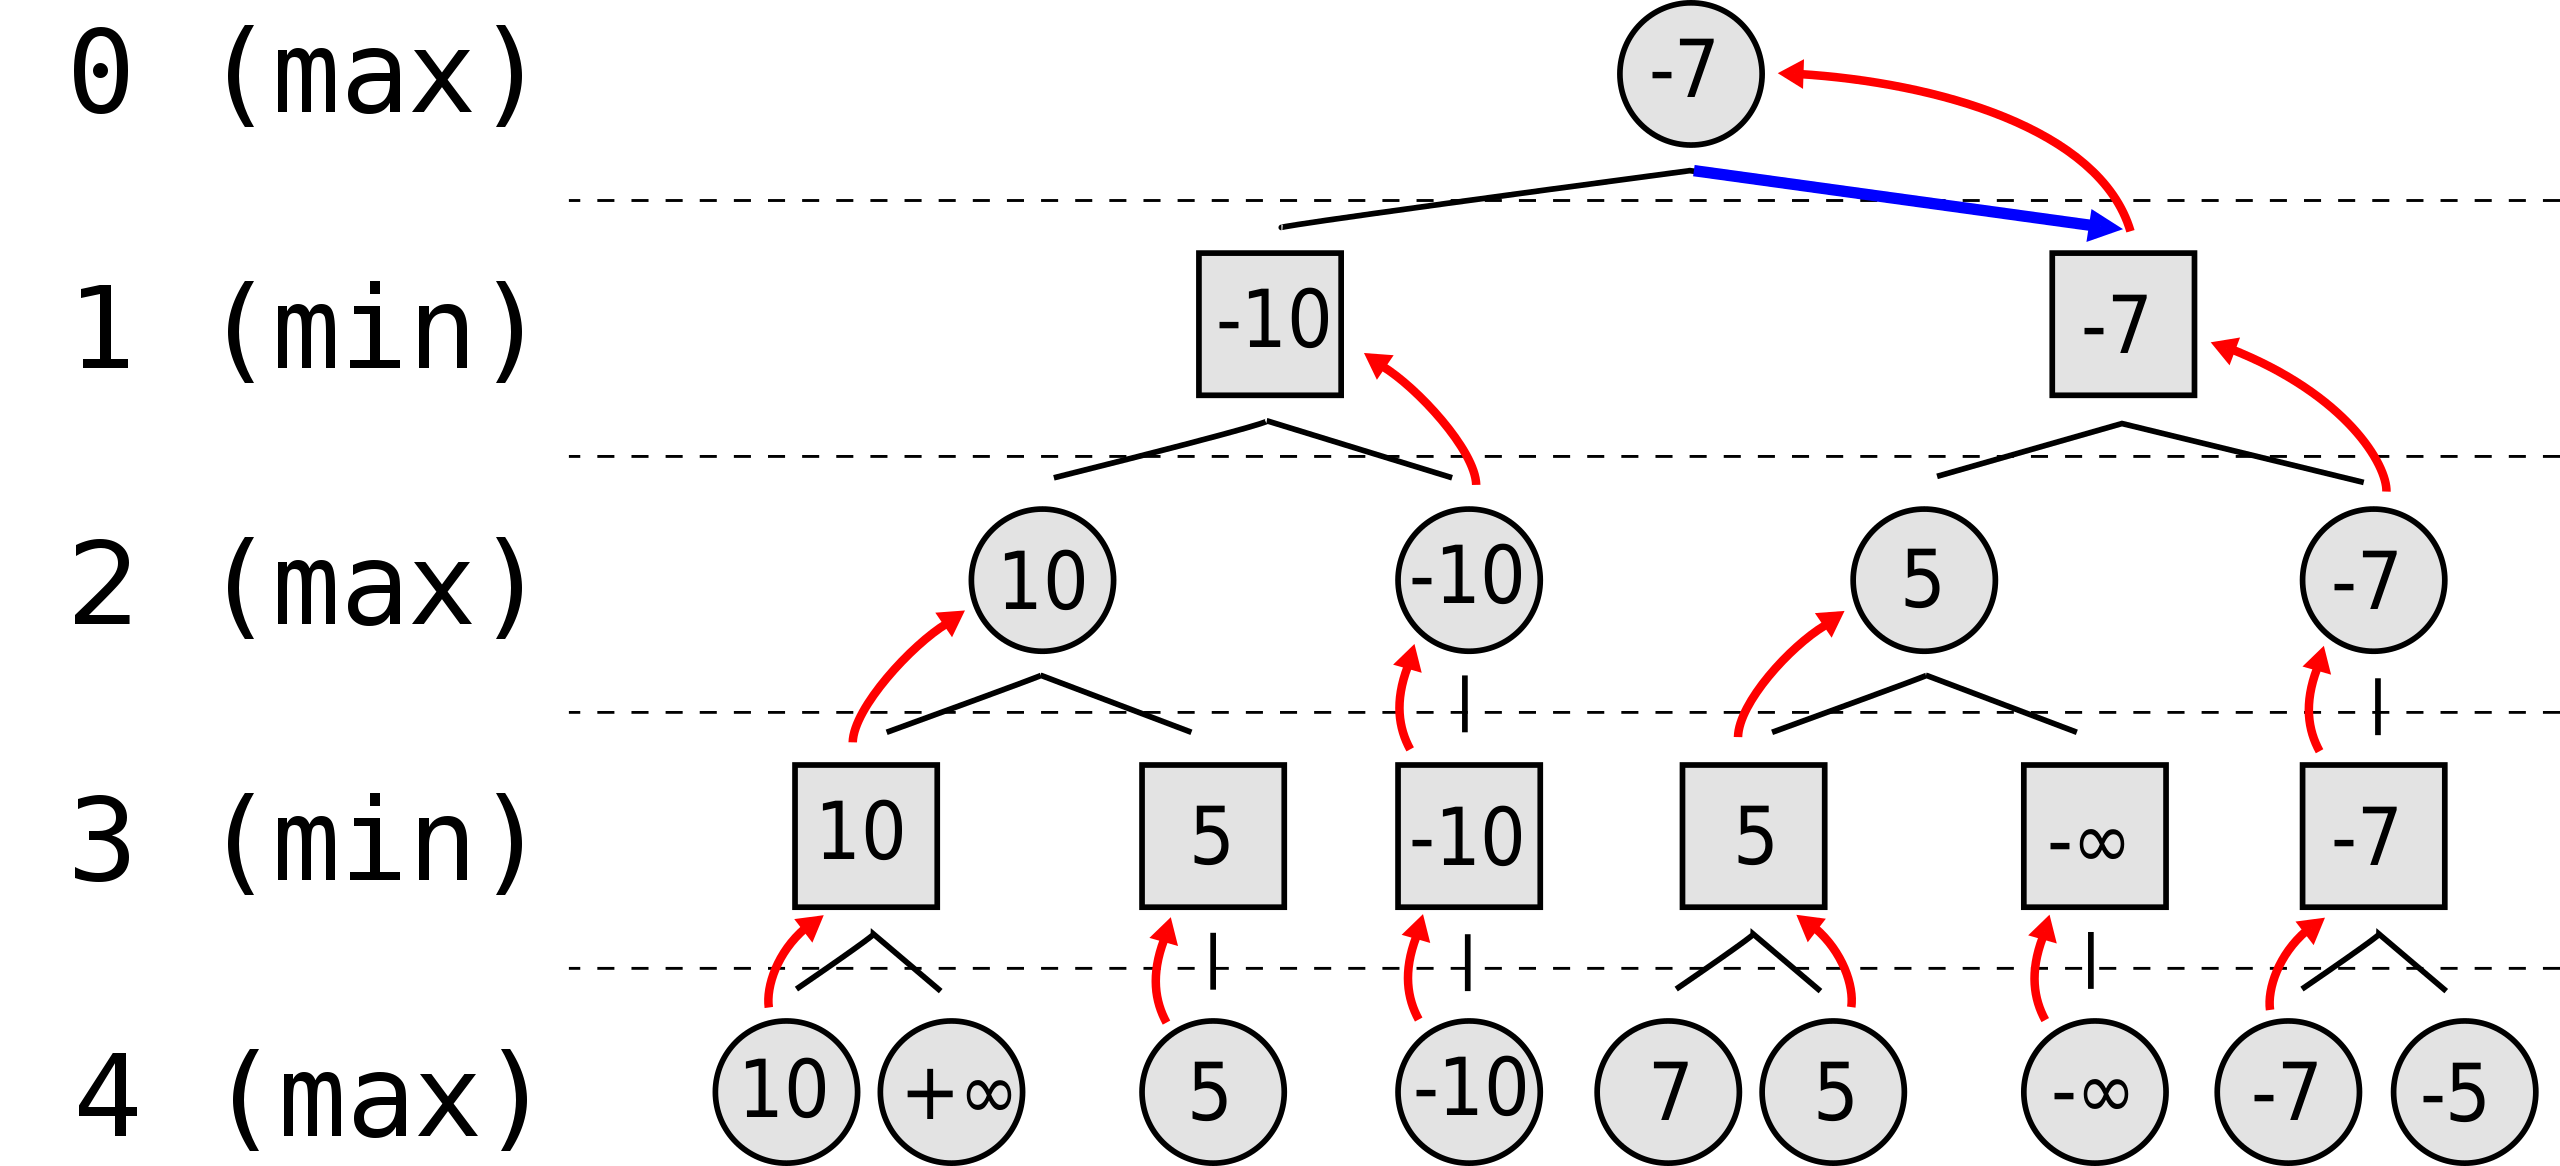
\includegraphics[width=0.6\textwidth]{Minimax.png}
    \caption[minimax]{%
      极小化极大算法搜索树例子\cite{wikiMinimax}%
      }
    \label{fig:minimax}
  \end{figure}

如图2.1所示,假设圆形代表当前选手,方形代表对手。当前选手需要将自己所得分数最大化,而对手则需要反其道行之。考虑第三层(Min层)对手在最左侧节点的决策,当前选手在第四层有得分为10或正无穷的行动选择,作为对手要做的是最小化这个分数,于是对手根据结果可以反推出应选择得分为10的行动。其余同理。
\subsection{Alpha-beta 剪枝}
在上一个小节中我们介绍了经典的极小化极大算法,对于一个具有复杂状态空间的游戏(象棋或围棋)来说,Minimax算法需要非常多层才能够完成。如果这个游戏每一步都有$n$个选择,那么在$x$步以后,将会有$n^x$个选择,也就是说具有指数级复杂度。在这种情况下,使用经典的极小化极大算法进行树搜索是不现实的。因此我们就需要采取剪枝来减少运算量,剪掉上述树状图的一些分支,从而减少运算量。

Alpha-beta剪枝用于裁剪搜索树中不需要搜索的节点。$\beta$值为可行解的最小上界(Min层通向root的路径上最好的选择),$\alpha$值为可行策略(解)的最大下界(Max层通向root的路径上最好的选择)。其在生成博弈树的同时计算评估各节点的$\alpha$值与$\beta$值, 并且根据评估出的值范围, 及时停止扩展那些已无必要再扩展的子节点,以提高运算速度。该算法和极小化极大算法所得结论相同,但剪去了不影响最终决定的分枝\cite{russell2010artificial}。
剪枝过程遵循$\alpha \le N \le \beta$,N为当前节点评估值。即:(1)当一个 Min 节点的 $\beta$值小于等于任何一个父节点的$\alpha$值时 ,剪掉该节点的所有子节点;(2)当一个 Max 节点的 $\alpha$值大于等于任何一个父节点的$\beta$值时 ,剪掉该节点的所有子节点。
我们用以下Minimax树(图2.1)作为例子,方块为Max节点,圆形为Min节点\cite{russell2010artificial}。
\begin{figure}[htb]
    \centering
    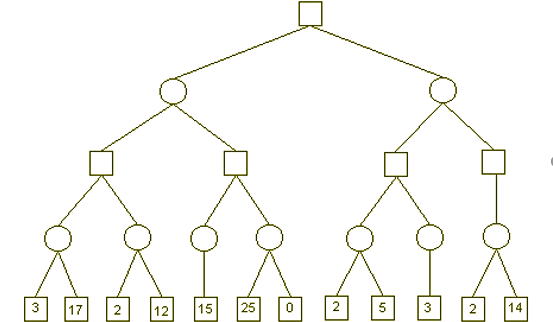
\includegraphics[width=0.6\textwidth]{abp1.PNG}
    \caption[abp]{%
    Alpha-beta剪枝初始状态\cite{russell2010artificial}%
      }
    \label{fig:abp}
  \end{figure}

其剪枝过程如图2.3所示。从左节点开始,

(1)当到达深度为4层处的第一个子节点时,在该状态上进行评估并获得值为3。将此节点值传递回上面的父Min节点。由于这是一个Min节点,因此该节点的Minimax值必须小于或等于3。换句话说,我们将该Min节点$\beta$值更改为3;

(2)接下来在深度为4层处遍历下一个子节点,并向父Min节点返回值17;

(3)由于父节点为Min节点,并且17大于3,因此将忽略返回17的子节点。 现在我们已经评估了这个Min节点的所有子节点,因此我们将$\beta$值返回到上面的Max节点。 Max节点的值将大于或等于3,因此我们将$\alpha$更改为3:

(4)遍历该Max节点的新Min子节点,并将当前的区间传递给子节点;

(5)搜索新Min子节点的子节点,第一个值为2并传递给Min父节点;

(6)父节点的值将小于或等于2,因此将其$\beta$值改为2;我们发现在此节点上找到解决方案路径的唯一方法是找到一个值大于3且小于2的子节点。由于这是不可能的,我们可以停止评估此节点的子节点,然后返回$\beta$值(也就是2)作为该节点的值。
回到父Max节点,其$\alpha$值已经是3,比2更具限制性,因此不要更改它。我们已经看到了此max节点的所有子节点,因此可以将其值设置为最终的$\alpha$值即为3。

\begin{figure}[htb]
    \centering
    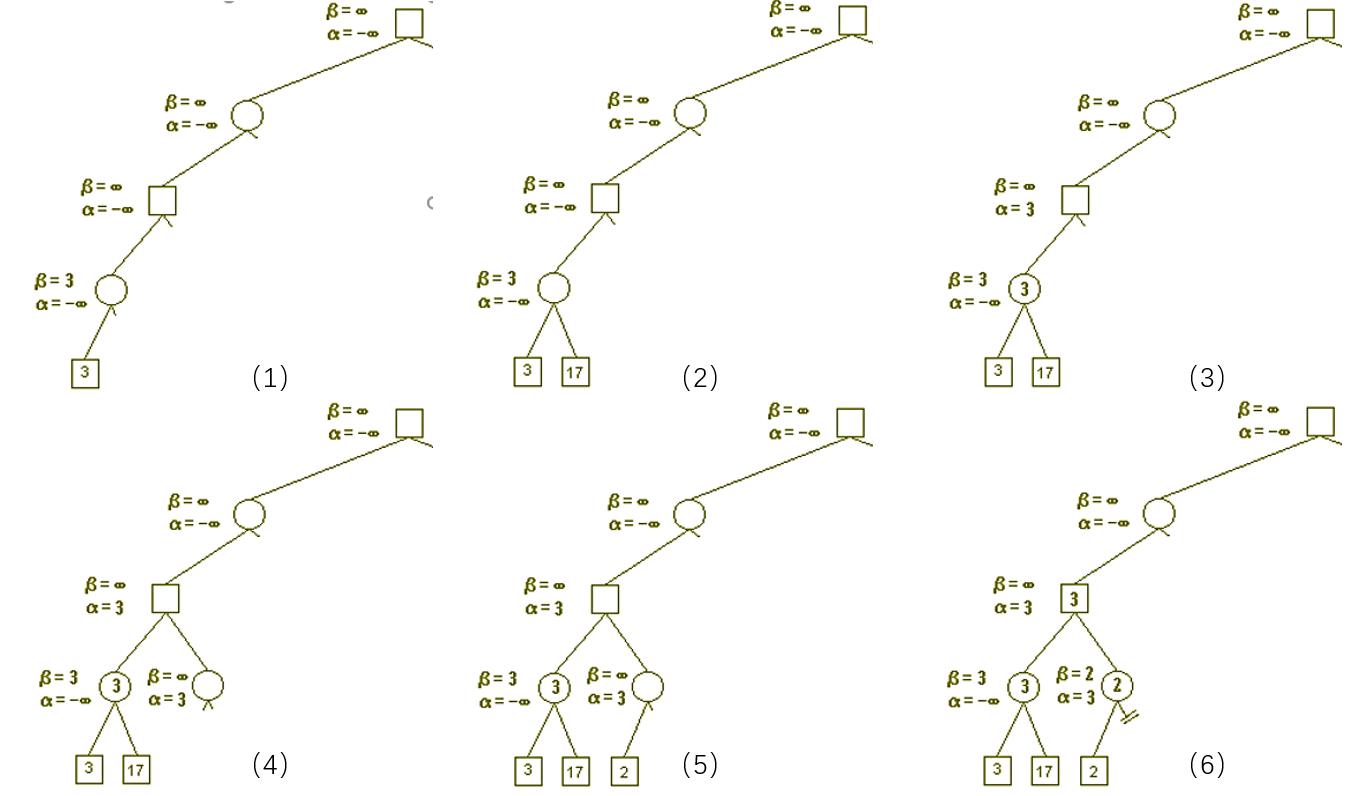
\includegraphics[width=0.9\textwidth]{abp2.PNG}
    \caption[abp2]{%
    Alpha-beta剪枝\cite{russell2010artificial}%
      }
    \label{fig:abp2}
  \end{figure}
\newpage
Alpha-beta剪枝是在极小化极大算法上的改进,减少搜索树的分枝,从而提升搜索深度。
若节点搜索顺序达到最优化或近似最优化(将最佳选择排在各节点首位),则同样时间内搜索深度可达极小化极大算法的两倍多\cite{KNUTH1975293abp}。但是对于较复杂的棋类游戏,若对AI的每一步有时间限制,Alpha-beta剪枝的搜索深度依然受到较大限制,在实际应用中往往采取3-4层,也有可能导致只能获得局部最优解。
除此之外,对手玩家一定会选择使自己最差的思路的先验假设,在真实情况下并不正确,因为无法确定对方的博弈策略是否和自己一致。如果对方做的策略不是最优,那么我方策略是最优的假设也不复存在。

\subsection{蒙特卡洛树搜索}
蒙特卡洛树搜索(Monte Carlo tree search,简称:MCTS)是一种启发式搜索算法,其在游戏树搜索的应用十分广泛\cite{10.1007/978-3-540-75538-8_7}。顾名思义,其设计思路是基于概率的:蒙特卡洛树搜索会多次模拟博弈过程,并尝试根据模拟结果预测最优的移动方案。这也与人类下棋时的思维模式符合:根据“棋感”在脑海里大致筛选出了几种最可能的走法,然后再想走了这几种走法之后对手最可能的走法,然后再想自己接下来最可能的走法。

蒙特卡洛树搜索的每个循环包括四个步骤\cite{RePEc:wsi:nmncxx:v:04:y:2008:i:03:n:s1793005708001094}:
(1)选择(Selection):从根节点R开始,选择连续的子节点向下至叶子节点L。选择子节点的方式一般采取上限置信区间算法(UCT)\cite{10.1007/11871842_29};
(2) 扩展(Expansion):除非任意一方的输赢使得游戏在L结束,否则创建一个或多个子节点并选取其中一个节点C;
(3)仿真(Simulation):在从节点C开始,用随机策略进行游戏,又称为playout或者rollout;
(4) 反向传播(Backpropagation):使用随机游戏的结果,更新从C到R的路径上的节点信息。
谷歌公司的AlphaGo/Zero体系中都使用了MCTS的架构并对其策略进行了改进与优化。

\begin{figure}[htb]
    \centering
    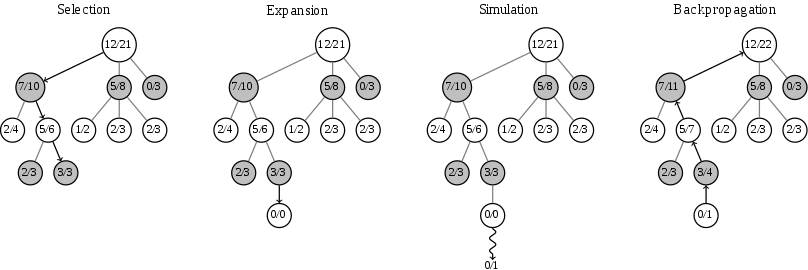
\includegraphics[width=0.9\textwidth]{mctswiki.png}
    \caption[mcts]{%
    蒙特卡洛树搜索的步骤,每一个节点的内容代表胜利次数/游戏次数\cite{RePEc:wsi:nmncxx:v:04:y:2008:i:03:n:s1793005708001094}%
      }
    \label{fig:mcts}
  \end{figure}
\newpage

\subsubsection{选择子节点的方式}


\section{卷积神经网络模型}

\subsection{深度残差网络}

\section{强化学习}

\subsection{基于策略的算法}

\subsection{基于值的算法}